\chapter{\label{chap:grundlagen}Grundlagen}
Dieses Kapitel befasst sich mit sowohl den mathematischen als auch den technischen Grundlagen der zu behandelnden Thematik, welche für das weitere Verständnis der Arbeit beitragen.
% -------------------------------------------------
% TECHNISCHE GRUNDLAGEN
% -------------------------------------------------
\section{\label{sec:technGrundlagen}Technische Grundlagen}
Im Zuge dieser Arbeit wird eine Smartphone Anwendung erstellt, deren Grundlage für die Implementierung die Software-Plattform Android und der im \gls{Smartphone} integrierte \gls{GPS}-Sensor ist. Die eigene Position und Geschwindigkeit wird mittels \gls{GPS} ermittelt, um in Verbindung mit der festen Position der nächsten \gls{LSA} die optimale Geschwindigkeit für das Erreichen der "'Grünen Welle"' zu errechnen. Im folgenden Abschnitt werden Funktionsweise und Besonderheiten der verwendeten Technologien beschrieben. 
% ANDROID
\subsection{Android}
Die umfassende Open-Source-Plattform Android stellt eine vollständige Ausstattung für Mobilgeräte dar. Android-Anwendungen werden mit der Programmiersprache Java und der Auszeichnungssprache \gls{XML} entwickelt. Mit dem Android \gls{SDK}\footnote{ Das Android \gls{SDK} steht unter \url{https://developer.android.com/sdk/index.html} zum Download bereit} werden die Werkzeuge und \gls{API} zur Verfügung gestellt, die erforderlich sind Mobilanwendungen auf der Android-Plattform erzeugen zu können.\\ 
Zu den wichtigsten \gls{SDK} Werkzeugen gehören der Android \gls{SDK}-Manager, der AVD-Manager, der Emulator und der Dalvik Debug Monitor Server(Ddms). Der \gls{SDK}-Manager verwaltet die \gls{SDK}-Pakete, sowie die installierten Pakete und System-Images. Der AVD-Manager bietet eine grafische Oberfläche in der Android Virtuell Devices verwaltet, und im Emulator ausgeführt werden können. Mithilfe des Ddms können Android Anwendungen auf Fehler untersucht werden. \cite{android_sdk} \\
Ursprünglich gab es die  Virtuelle Maschine Dalvik, die unter Berücksichtigung von Rechenleistung und der Lebensdauer von Batterien speziell für Android entworfen wurde. [\textsc{Quelle}]
Diese wurde mit Android 5.0 von der Android Runtime (ART) als effizientere Laufzeit komplett ersetzt. \cite{android_5}\\\\
Mit dem Android \gls{NDK}\footnote{ Das Android \gls{NDK} steht unter \url{https://developer.android.com/tools/sdk/ndk/index.html} zum Download bereit} existiert auch ein Tool, mit dem Teile einer Anwendung in systemeigenen Programmiersprachen wie C oder C++ implementiert werden können. Programmcode der in solchen Sprachen geschrieben ist, eignet sich zum Beispiel bei CPU-intensiven Operationen wie Signalverarbeitungen oder Physik-Simulationen besonders gut. Hier ist allerdings sicherzustellen, ob die erforderlichen Bibliotheken in dem \gls{SDK} auch verfügbar sind. \cite{android_ndk} \\
Einen Überblick über die komplexe Android-Systemarchitektur, welche nachfolgend (nach \cite{android} S. 3ff) kurz beschrieben wird, zeigt die folgende Abbildung.
\begin{figure}[H]  
    \centering  
    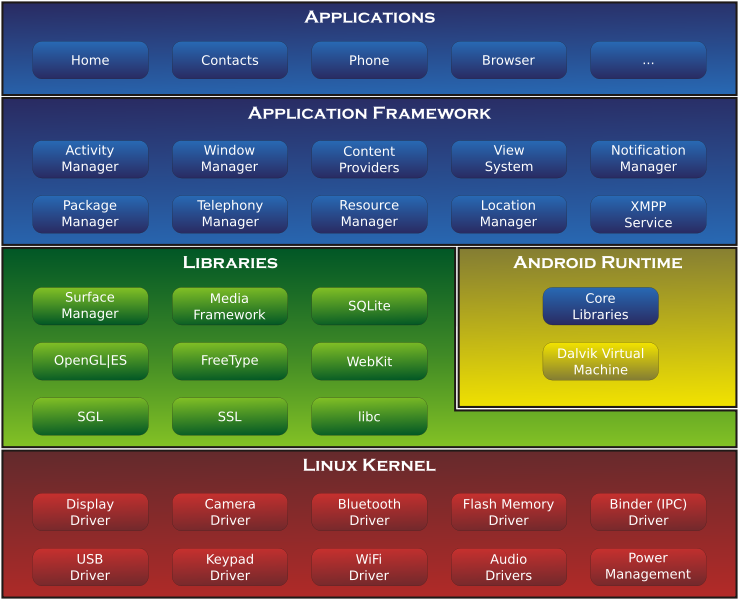
\includegraphics[width=0.7\textwidth]{Android-System-Architecture} 
    \caption[Android-Systemarchitektur]{Die Android-Systemarchitektur Quelle: \url{http://en.wikipedia.org/wiki/File:Android-System-Architecture.svg}}
    \label{fig:android}
\end{figure}
\paragraph{Linux Kernel: }
Android basiert auf dem Linux 3.1-Kernel. Dieser eine bewährte Betriebssystemgrundlage indem er die erforderlichen Hardware-Treiber zur Verfügung stellt.
\paragraph{Bibliotheken: }
Systemeigenen Bibliotheken sind C/C++ Bibliotheken und vorinstalliert. Dazu gehören alle Bibliotheken im grünen Bereich von Abbildung \ref{fig:android}:
\begin{itemize}[leftmargin=0.7cm]
\renewcommand\labelitemi{--}
	\item \textsc{Surface Manager} ~ Der für die Displayverwaltung verantwortliche Oberflächen-Manager
	\item \textsc{OpenGL/ES} ~ Eine 2D und 3D Grafikbibliothek
	\item \textsc{SGL} ~ Eine 2D Grafikbibliothek
 	\item \textsc{Media-Framework} ~ eine Medien-Bibliothek zur Wiedergabe von Audio- und Video-Daten 	
 	\item \textsc{FreeType} ~ eine Bibliothek zur Darstellung von Computerschriften als Rastergrafik
 	\item \textsc{SSL} ~ Das Secure-Socket-Layer für die Internet-Sicherheit
	\item \textsc{SQLite} ~ Ist eine ausgereifte Datenbank die den internen Speicher nutzt 
	\item \textsc{Webkit} ~ WebKit ist die Standard-Browser-Engine und erlaubt das schnelle Rendern und Anzeigen von HTML Seiten
	\item \textsc{libc} ~ C-Bibliothek
\end{itemize}
\paragraph{Android Runtime: }
Die Android Laufzeitumgebung nutzt die Java-Core-Bibliotheken und bis zur Version 5.0 auch die Dalvik \gls{VM}, weswegen diese noch auf der Grafik abgebildet ist.  
\textit{Die Dalvik \gls{VM} ist Googles Implementation von Java, zur Anwendung auf mobilen Geräten optimiert. Jede gestartete Android-Anwendung läuft in einem eigene Prozess und bekommt darüber hinaus seine eigene Dalvik \gls{VM}. Da die Anwendungen über keinen gemeinsamen Speicher verfügen erhöht das die Sicherheit und Verfügbarkeit und ist somit optimaler, obwohl mehr Ressourcen benötigt werden. Denn ein sterbender Prozess nimmt so nur seine "'eigene"' Anwendung mit. \\ 
Die Anwendungen werden zunächst von einem normalen Java-Compiler in Java-Bytecode übersetzt und dann von dem Dex-Compiler in den Dalvik-Bytecode, welcher schließlich von der Dalvik \gls{VM} ausgeführt wird. \cite{android_art}}
\paragraph{Application Framework: }
Androids Application-Framework ist eine Umgebung die unterschiedliche Dienste zur Verfügung stellt. Sie bietet EntwicklerInnen Zugriff auf die im Kern verwendeten \glspl{API} sowie auf die Java-Bibliotheken die für Android erstellt wurden. 
\paragraph{Applications: }
Auf der obersten Ebene in Abbildung \ref{fig:android} befinden sich die Anwendungen die den täglichen Telefon-Bedarfs wie Adressbuch, Messenger, E-Mail, Internet-Browser etc. decken. Zusätzlich unterstützt Android verschiedene Anwendungen von Drittanbietern. Diese sind hauptsächlich in Java geschrieben und werden am häufigsten über den Google Play Store verteilt.
\subsection{Die native Datenbank SQLite}
% MOBILE SENSING
\subsection{Mobile Sensorik <-- Ich benutze nur GPS?} 
Ein Sensor\footnote{ aus dem Lateinischen, deutsch: "'\textit{fühlen}"'} ist ein Bauelement, das physikalische Eigenschaften wie Helligkeit, Temperatur oder Beschleunigung sowohl quantitativ als auch qualitativ erfassen kann.
Die \gls{GPS}-Sensoren in \glspl{Smartphone} sind kostengünstiger, kleiner und haben einen geringeren Stromverbrauch. Dafür allerdings eine geringere Messgenauigkeit. In der zu entwickelnden Anwendung kommt es auf jeden Meter an. Ob die Genauigkeit des integrierten \gls{GPS}-Sensors genügt, muss also im Rahmen dieser Arbeit getestet werden. 
\subsubsection{Mobile Sensorik unter Android}
Die meisten Android-Mobilgeräte verfügen über integrierte Sensoren, die die Bewegung, Ausrichtung und verschiedene Umgebungsbedingungen messen. Diese Sensoren sind praktisch wenn man dreidimensionale Gerätbewegungen, Positionierungen oder Änderungen in der Umgebung des Gerätes überwachen möchte. So können zum Beispiel Spieleanwendungen den Beschleunigungssensor nutzen, um komplexe BenutzerInnengesten und Bewegungen wie Neigung, Erschütterung, Drehung oder Schwenkung erfassen.\\
Die Android-Plattform unterstützt Bewegungssensoren zum Messen von Beschleunigungen und Drehungen in drei Achsen, Umgebungssensoren zur Ermittlung verschiedener Umweltparameter wie Luftdruck und -feuchtigkeit, oder Beleuchtung und Temperatur, und Positionssensoren zum Messen der physikalischen Position des Gerätes. Android bietet mit dem Android Sensor Framework eine Sammlung von Klassen und Schnittstellen an mithilfe dessen man diese Sensoren zugreifen und deren Daten erfassen kann. \cite{android_sensor} 
\subsubsection{Geolokation mittels \gls{GPS}}
\gls{GPS} gewährleistet die Bestimmung des exakten Standpunktes und ist so wesentlicher Bestandteil ortsgebundener Anwendungen wie zum Beispiel die in Kapitel \ref{chap:state} beschriebenen. \\
Funktionsweise: Position und Geschwindigkeit können aus Signallaufzeiten zwischen Satelliten und EmpfängerIn bestimmt werden.\\
Android unterstützt mit dem \texttt{android.location} Paket den Zugriff auf die Ortungsdienste. Als zentrale Komponente des Location Frameworks stellt der \texttt{LocationManager} \glspl{API} zur Lokalisierung des Geräts bereit. Mit dem \texttt{LocationManager} ist die Anwendung in der Lage alle Location Provider\footnote{ deutsch: Standortanbieter. Ein Standortanbieter bietet regelmäßige Berichte über die geographische Lage des Gerätes} des letzten bekannten Standortes abzufragen, sich für regelmäßige Updates zur Position des Gerätes anzumelden und sich wieder abzumelden wenn sich das Gerät außerhalb gegebener Parameter befindet.
\cite{android_gps}
%\subsubsection{G-Sensor}Blabla Beschleunigungssensor...\\  Anwendungsbeispiel: um Bewegungsänderungen festzustellenß\\ Messprinzip: misst die Kraft, die auf die Masse im Sensor wirkt (F=m*a)\\Sensormasse ist bekannt, die Beschleunigung kann also bestimmt werden.Hohe Messgeschwindigkeit \\ Smartphone Sensoren sind potentiell für die Schlaglochdetektion geeignet
\clearpage
% -------------------------------------------------
% MATHEMATISCHE GRUNDLAGEN
% -------------------------------------------------
\section{\label{sec:mathGrundlagen}Berechnung der Geschwindigkeitsempfehlung}
Präsentiert das System während der Anwendung eine Geschwindigkeitsempfehlung, ist diese abhängig von der Fahrtgeschwindigkeit und vom Abstand zur Ampel. Angenommen die Progressionsgeschwindigkeit $v$ wird zum Zeitpunkt $t_{1}$ ermittelt, die \gls {LSA} schaltet zum Zeitpunt $t_{2}$ auf Rot und Abstand zur Ampel beträgt $s$, dann gilt: \\
\[ v = \frac{s}{t_{2} - t_{1}} \] \\
Der Abstand zur Ampel wird also durch die verbleibende Zeit dividiert. 
Die von der Berliner Verkehrsleitzentrale zur Verfügung gestellten Ampelschaltpläne und Position der angesteuerten Ampel dienen als Grundlage dieser Berechnung und sind aus der Datenbank zu holen. Die aktuelle Position des Fahrrads wird vom \gls{GPS} Sensor des \glspl{Smartphone} ermittelt und daraus der Abstand zur Ampel errechnet. Die Abbildung \ref{fig:vst} soll die Berechnungsgrundlagen veranschaulichen: 
\begin{figure}[H]  
    \centering  
    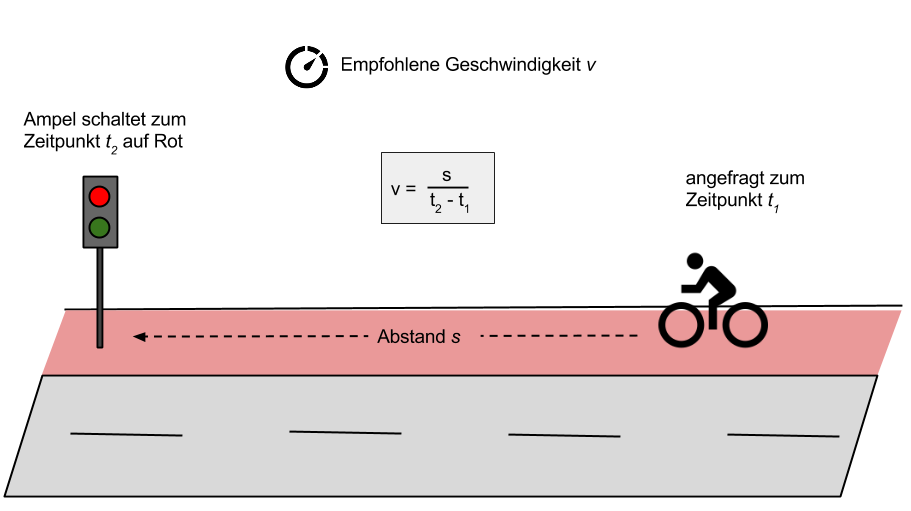
\includegraphics[width=1\textwidth]{vst}     
    \caption[Berechnung Progressionsgeschwindigkeit]{Veranschaulichung der Berechnung}
    \label{fig:vst}
\end{figure}
Um die ensprechende \gls{LSA} während der Grünphase zu passieren, muss letztendlich die empfohlene Geschwindigkeit $v$ eingehalten werden.
